\begin{XeClass}{DU}
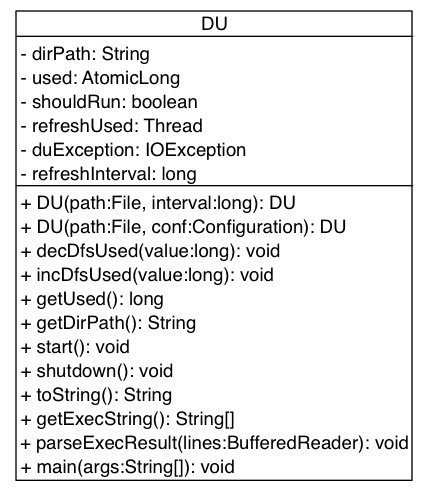
\includegraphics[width=\textwidth]{cdig/DU.png}
     
 文件夹的磁盘使用状态.
 继承自\emph{org.apache.hadoop.util.Shell},在Shell中调用系统工具
 使用\emph{du -sk <path>}实现,该命令无法在Windows环境下使用
 在Windows环境下使用\emph{dir <path>}能得到相关信息,但无关的输出过多
 内部使用一个线程定期执行命令刷新状态

    \begin{XeMethod}{\XePublic}{DU}{DU}
         
 设置磁盘监控的路径以及时间间隔,开始保持对磁盘使用量的监控,

    \end{XeMethod}

    \begin{XeMethod}{\XePublic}{void}{decDfsUsed}
         
 减少系统预留的磁盘空间

    \end{XeMethod}

    \begin{XeMethod}{\XePublic}{void}{incDfsUsed}
         
 增加系统预留的磁盘空间

    \end{XeMethod}

    \begin{XeMethod}{\XePublic}{long}{getUsed}
         
 返回磁盘使用量

    \end{XeMethod}

    \begin{XeMethod}{\XePublic}{String}{getDirPath}
         
 返回被监控的路径

    \end{XeMethod}

    \begin{XeMethod}{\XePublic}{void}{start}
         
 开启一个进程,来监控磁盘使用

    \end{XeMethod}

    \begin{XeMethod}{\XePublic}{void}{shutdown}
         
 关闭刷新线程

    \end{XeMethod}

    \begin{XeMethod}{\XeProtected}{String[]}{getExecString}
         
 检测命令

    \end{XeMethod}

    \begin{XeMethod}{\XeProtected}{void}{parseExecResult}
         
 解析输出

    \end{XeMethod}

    \begin{XeInnerClass}{DURefreshThread}
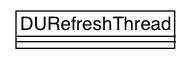
\includegraphics[width=\textwidth]{cdig/DURefreshThread.png}
         
 刷新线程

    \end{XeInnerClass}
\end{XeClass}
